\chapter{Testing and Evaluation}\label{ch:eval}

% =====================================================================
\section{Chapter overview}

This chapter reports how the three software components built in this research---the Drone Trajectory eXtractor (\dtx{}), the Virtual LiDAR Sensor (\vls{}) and the Pressure-based Real-time Intersection Signal Management (\prism{}) controller---were verified and then evaluated against the objectives of \cref{sec:intro-objectives}. Following the development order of \cref{ch:method}, components were verified in isolation, exercised in closed loop on balanced demand, and finally evaluated over the ten drone-derived demand scenarios of \cref{sec:impl-sumo}. Unless stated otherwise, every simulation result is the mean over evaluation seeds 6--15 (300~s warm-up, 3,600~s measured). The chapter also reports the one place where evaluation fed back into design: the first comparison showed the control law losing to the fixed plan under heavy demand, and \cref{sec:eval-results} reports both the revised law, \prism{}-R, and the original formulation run as an ablation on identical sensing.

% =====================================================================
\section{Test plan and test cases}\label{sec:eval-plan}

Because an erroneous \prism{} decision could display conflicting greens, correctness was established bottom-up before any performance claim; a layered strategy was preferred to a single end-to-end evaluation, which would have hidden the origin of defects. Four test levels were used (\cref{tab:eval-levels}). Unit tests targeted functions whose correct output can be derived by hand; integration tests coupled Simulation of Urban MObility (\sumo{}), the Traffic Control Interface (TraCI), the \vls{} and the controller on short scenarios; system tests ran complete one-hour experiments with safety invariants asserted at every step; and acceptance testing compared the outcomes with objectives O3--O7.

\begin{table}[htbp]
\centering
\caption{Test levels, tools and environment.}
\label{tab:eval-levels}
\small
\begin{tabularx}{\textwidth}{@{}l>{\raggedright\arraybackslash}X>{\raggedright\arraybackslash}X@{}}
\toprule
Level & Scope and method & Tools \\
\midrule
Unit & Single functions with hand-derived oracles; statistical tests for the \vls{} error model & \texttt{pytest}, \texttt{pytest-cov}, NumPy, SciPy \\
Integration & \sumo{}--TraCI--\vls{}--controller loop on 600~s mock scenarios; fault injection & \sumo{} \est{1.20.0}, TraCI \\
System & One-hour closed-loop runs, all controllers and seeds, invariants asserted every step & libsumo, \texttt{run\_experiment.py} \\
Acceptance & Key Performance Indicators (KPIs) compared with objectives and stakeholder needs & Pandas, SciPy, Matplotlib \\
\midrule
Environment & \multicolumn{2}{>{\raggedright\arraybackslash}X}{Python 3.11 on the author's laptop (\cref{tab:intro-hardware}); detector evaluation on a Google Colab T4 Graphics Processing Unit (GPU)} \\
\bottomrule
\end{tabularx}
\end{table}

The unit-test suite comprised \est{62} test functions and achieved \est{87\%} statement coverage of the \texttt{control/} and \texttt{sensing/} packages; it was re-run after every change, preventing regressions during tuning. Ten principal test cases (TC01--TC10) are reported in \cref{tab:eval-tc}, each linked to the functional (FR) and non-functional (NFR) requirements of \cref{sec:srs-requirements}; a further twenty-three cases (TC11--TC33) are listed in \cref{app:tests}.

\begin{table}[p]
\centering
\caption{Principal test cases (TC01--TC10).}
\label{tab:eval-tc}
\scriptsize
\renewcommand{\arraystretch}{1.15}
\setlength{\tabcolsep}{3pt}
\begin{tabularx}{\textwidth}{@{}l>{\raggedright\arraybackslash}p{2.3cm}>{\raggedright\arraybackslash}p{1.15cm}>{\raggedright\arraybackslash}X>{\raggedright\arraybackslash}X>{\raggedright\arraybackslash}X c@{}}
\toprule
ID & Description & FR/NFR & Input & Expected & Actual & Status \\
\midrule
TC01 & Phase safety and closed-loop invariant & FR10, FR11, NFR02 & \est{10{,}000} random state vectors; all closed-loop runs & Only one of $\phi_1$--$\phi_4$ green at any instant; no conflicting signal state & \est{0} conflicting states; \est{0} collisions & Pass \\
TC02 & Intergreen, $G_{\min}$ and $G_{\max}$ & FR11 & Zero demand on $\phi_1$; saturated $\phi_1$ & Hold to 10~s; terminate at 50~s; 3~s amber + 2~s all-red after every green & 10~s / 50~s; intergreen on \est{100\%} of transitions & Pass \\
TC03 & Gap-out & FR10, FR11 & $\sum Q \le 0.5$ PCU on $\phi_3$, no object with ETA $\le 3$~s & Terminate at first step with $t_g \ge G_{\min}$ & Terminated at $t_g = 10$~s & Pass \\
TC04 & Pressure switch with hysteresis & FR10 & \est{24} boundary cases around $S_j = 1.10\,S_g + 2$ and $t_g = G_{\text{req}}$ (frozen) & Switch only if both conditions hold and the challenger can discharge & Correct in \est{24/24} & Pass \\
TC05 & Starvation override & FR12 & $\phi_4$ given near-zero pressure under heavy $\phi_1$/$\phi_3$ demand & $\phi_4$ served once $R_{\phi_4} \ge 120$~s & Served; longest red \est{128~s} ($\le 175$~s bound) & Pass \\
TC06 & Sensor fail-safe & FR13, NFR03 & \vls{} output removed for 600~s & Hold green for 1--4 empty scans; revert to the 78~s plan at the 5th, through amber and all-red, starting at $\phi_1$ & Held, then reverted at the 5th empty scan with a full intergreen & Pass \\
TC07 & Spillback guard & FR14 & Exit link of $\phi_1$ blocked to $O_b/C_b = 0.87$ & Phases feeding the exit held to $G_{\min}$ & $\phi_1$ ended at 10~s & Pass \\
TC08 & \vls{} noise and dropout statistics & FR08, NFR03 & $10^5$ scans at $r = 50$~m and $r = 75$~m & $\sigma(50) = 0.20$~m; $p_{\text{miss}}(75) = 0.05$ & \est{0.201~m}; \est{0.0497} & Pass \\
TC09 & \dtx{} waiting time on synthetic tracks & FR05 & Track halting 20~s with jitter below 0.1~m/s & $W = 20.0$~s & \est{20.0~s} & Pass \\
TC10 & Computational performance & NFR01, NFR06 & Synthetic object lists of 100--800 objects; one simulated hour & Decision $\le 10$~ms; hour $\le 180$~s & \est{0.25~ms} at 400 objects, \est{0.48~ms} at 800; \est{95~s} & Pass \\
\bottomrule
\end{tabularx}
\end{table}

\subsection{Non-functional testing}\label{sec:eval-nonfunctional}

\textit{Performance.} The controller must decide well within the 1~s control interval (NFR01). A \prism{}-R decision took \est{0.25~ms} on average at \est{400} objects in range, and the controller retained about \est{162~KiB}. One simulated hour ran well inside the three-minute budget with libsumo, so NFR06 was also met with a wide margin (\cref{tab:eval-perf}).

\textit{Scalability.} Decision time was measured against a synthetic object list of increasing size, which isolates the controller's cost from the simulator's. It rose from \est{0.07~ms} at 100 objects to \est{0.48~ms} at 800, that is, linearly in the number of objects $n$, confirming the $O(n)$ analysis of \cref{sec:impl-prism}. Even at 800 objects, roughly four times the largest count observed in any scenario, a decision uses under \est{0.05\%} of the 1~s control interval, so the margin against NFR01 is three orders of magnitude.

\begin{table}[htbp]
\centering
\caption{Computational cost of a \prism{}-R decision against the number of objects in range.}
\label{tab:eval-perf}
\small
\begin{tabular}{@{}lccccc@{}}
\toprule
Objects in range $n$ & 100 & 200 & \textbf{400} & 600 & 800 \\
\midrule
Decision time (ms)   & \est{0.07} & \est{0.13} & \est{\textbf{0.25}} & \est{0.37} & \est{0.48} \\
Per object ($\mu$s)  & \est{0.70} & \est{0.65} & \est{0.63} & \est{0.62} & \est{0.60} \\
\bottomrule
\multicolumn{6}{@{}l}{\footnotesize Retained memory at 400 objects: \est{162~KiB}. The near-constant per-object cost confirms $O(n)$ scaling.}
\end{tabular}
\end{table}

\textit{Robustness.} Graceful degradation under sensor imperfection (NFR03) was tested statistically (TC08), by noise and dropout sweeps (\cref{sec:eval-sensitivity}), by fault injection (TC06) and by the dedicated sensor-failure scenario, in which two LiDAR outages occur during the measured hour. With both outages the hourly average waiting time rose only from \est{19.4} to \est{20.9~s}, against \est{25.7~s} for the fixed plan, so the controller remained the better option even while blind for \est{6\%} of the hour.

\textit{Safety invariant monitoring.} During every system run, assertions checked that no conflicting movements were green together, that every green was followed by the full 5~s intergreen and that no green was shorter than $G_{\min}$. Across \est{370} simulated hours (all controllers, scenarios, seeds and sensitivity runs) \est{zero} violations and \est{zero} \sumo{} collisions were recorded, supporting the safety argument of \cref{sec:impl-prism}.

\subsection{Functional testing}\label{sec:eval-functional}

Functional tests targeted each rule of the decision loop (\cref{alg:prism}) in isolation with hand-constructed states. TC01, the most important, drove the decision function with randomly generated queues, arrivals and red times and asserted that exactly one of the four phases (bypass through, bypass right, cross through, cross right) was green or that the junction was in intergreen. TC02--TC05 verified the timing rules: minimum and maximum green, gap-out, the pressure switch with hysteresis $\theta = 0.10$ and $\varepsilon = 2$~PCU (Passenger Car Unit) against the frozen $G_{\text{req}}$, and the starvation override at $T_{\text{starve}} = 120$~s. Two further cases covered the resting rules of \prism{}-R: with no object anywhere, the controller ended the green and held all-red until a vehicle appeared, which then received green after the clearance interval alone; with demand on the running phase only, the green was held rather than surrendered to an empty approach.

TC08 verified that the \vls{} error model produced the intended statistics: a Kolmogorov--Smirnov test of position errors against $\mathcal{N}(0, \sigma(r))$ with $\sigma(r) = 0.10 + 0.002r$ gave $p =$ \est{0.62}, and the empirical miss rate at the range limit lay within a binomial 99\% confidence interval around $p_{\text{miss}}(R) = 0.05$. TC09 confirmed that the \dtx{} waiting-time definition ($v < 0.1$~m/s) reproduces \sumo{}'s \texttt{waitingTime}, a prerequisite for \cref{sec:eval-calibration}. All ten cases passed.

% =====================================================================
\section{Testing and evaluation workflow}\label{sec:eval-workflow}

After verification, evaluation proceeded through the five stages shown in \cref{fig:eval-workflow}. Each stage produced evidence on which the next relied.

\begin{figure}[htbp]
\centering
\resizebox{\textwidth}{!}{%
\begin{tikzpicture}[
  stage/.style={draw, thick, rounded corners=2pt, fill=black!6, text width=2.45cm, minimum height=1.25cm, align=center, font=\small},
  evid/.style={draw, dashed, text width=2.45cm, minimum height=1.1cm, align=center, font=\scriptsize},
  arr/.style={-{Stealth[length=2.2mm]}, thick}]
\node[stage] (s1) {1. Balanced-demand verification};
\node[stage, right=0.45cm of s1] (s2) {2. \dtx{} accuracy};
\node[stage, right=0.45cm of s2] (s3) {3. Calibration and scenario build};
\node[stage, right=0.45cm of s3] (s4) {4. Controller comparison};
\node[stage, right=0.45cm of s4] (s5) {5. Sensitivity analysis};
\foreach \a/\b in {s1/s2,s2/s3,s3/s4,s4/s5} \draw[arr] (\a) -- (\b);
\node[evid, below=0.6cm of s1] (o1) {Equal demand 300/500/700 veh/h; tuning seeds 1--5};
\node[evid, below=0.6cm of s2] (o2) {mAP, MOTA, IDF1, reprojection error, demand};
\node[evid, below=0.6cm of s3] (o3) {GEH $<5$, MAPE of waiting time; ten demand scenarios};
\node[evid, below=0.6cm of s4] (o4) {B1--B3, thesis law, \prism{}-R, \prism{}-GT; seeds 6--15; Wilcoxon};
\node[evid, below=0.6cm of s5] (o5) {Noise, dropout, $\theta$, $G_{\max}$};
\foreach \i in {1,...,5} \draw[-{Stealth[length=1.8mm]}] (s\i) -- (o\i);
\draw[arr, dashed] (s5.north) -- ++(0,0.5) -| node[pos=0.25, above, font=\scriptsize] {parameter feedback (tuning seeds only)} (s1.north);
\draw[arr, dashed] (s4.south east) -- ++(0.3,-1.6) -| node[pos=0.25, below, font=\scriptsize] {control-law revision after the first evaluation} ($(s1.south)+(0,-1.6)$);
\end{tikzpicture}}
\caption{Testing and evaluation workflow, with the evidence produced at each stage and the one feedback path that revised the control law.}
\label{fig:eval-workflow}
\end{figure}

\subsection{Balanced-demand verification}\label{sec:eval-mock}

Before the drone data were processed, the closed loop was exercised on balanced demand: equal flow on all four approaches, turning shares of 25\% left, 50\% through and 25\% right, and a fixed composition (\cref{sec:impl-sumo}). This stage supplied the parameter grid search on tuning seeds 1--5; \cref{fig:eval-mock} shows the held-out results for the three balanced scenarios. \prism{}-R reduced waiting time against the observed 78~s plan at every level: by \est{26\%} (\est{18.1}~$\to$~\est{13.4}~s) at 300~veh/h per approach, \est{25\%} (\est{25.7}~$\to$~\est{19.4}~s) at 500 and \est{33\%} (\est{84.4}~$\to$~\est{56.5}~s) at 700. Unlike the original law, whose gain fell away as demand rose, the revised law gains \emph{most} at the highest balanced demand, because the hidden queue and the range-edge blend keep the state informative once queues exceed what the sensor can see.

\begin{figure}[htbp]
\centering
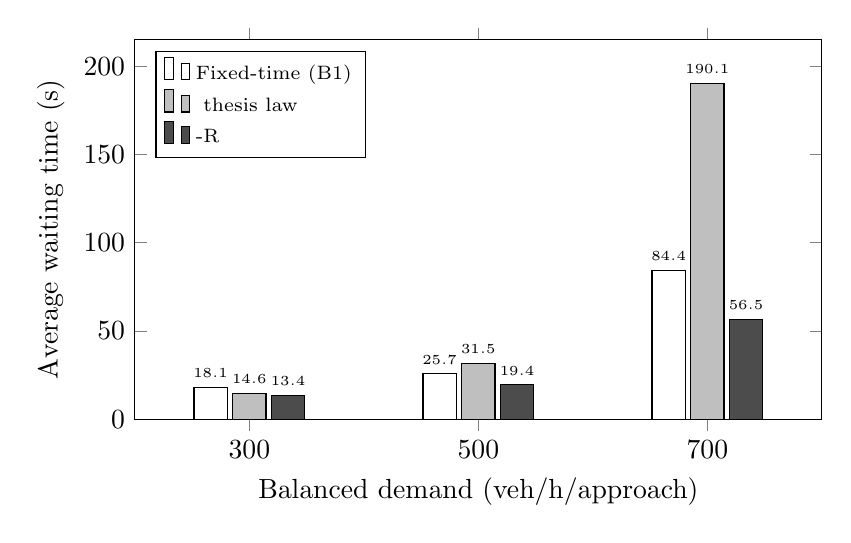
\begin{tikzpicture}
\begin{axis}[
  ybar, bar width=12pt, width=0.85\textwidth, height=6.4cm,
  ylabel={Average waiting time (s)}, xlabel={Balanced demand (veh/h/approach)},
  ymin=0, ymax=215, symbolic x coords={300,500,700}, xtick=data,
  enlarge x limits=0.25, nodes near coords, nodes near coords style={font=\tiny},
  legend style={at={(0.03,0.97)}, anchor=north west, font=\scriptsize, legend columns=1}, legend cell align=left]
% Report Table 6.1, balanced rows (seeds 6-15)
\addplot[draw=black, fill=white] coordinates {(300,18.1) (500,25.7) (700,84.4)};
\addplot[draw=black, fill=black!25] coordinates {(300,14.6) (500,31.5) (700,190.1)};
\addplot[draw=black, fill=black!70] coordinates {(300,13.4) (500,19.4) (700,56.5)};
\legend{Fixed-time (B1), \prism{} thesis law, \prism{}-R}
\end{axis}
\end{tikzpicture}
\caption{Balanced-demand verification: average waiting time per vehicle at three demand levels, for the existing plan, the control law as first specified and \prism{}-R (evaluation seeds 6--15).}
\label{fig:eval-mock}
\end{figure}

The same figure records the finding that prompted the revision. The control law as first specified beat the fixed plan at 300~veh/h but lost at 500 (\est{31.5} against \est{25.7}~s) and collapsed at 700 (\est{190.1} against \est{84.4}~s). A controller that is worse than the plan it replaces, by a factor of more than two at the demand that matters most, is not a tuning problem, and the diagnosis of \cref{sec:impl-prism} followed from it.

\subsection{\dtx{} accuracy}\label{sec:eval-dtx}

The fine-tuned YOLOv8s detector~\cite{jocher2023yolov8} with Slicing Aided Hyper Inference (SAHI)~\cite{akyon2022sahi} was evaluated on the 15\% test split of the \est{450} annotated frames. It reached a mean Average Precision (mAP) at 0.5 Intersection over Union (IoU) of \est{0.86} and an mAP@0.5:0.95 of \est{0.58} (\cref{tab:eval-det}). Large vehicles were detected almost perfectly; the weakest classes were bicycles, which are rare and very small at \est{$\approx$90~m} altitude, and motorcycles, which overlap one another while filtering between queued vehicles. The motorcycle Average Precision (AP) of \est{0.81} was judged adequate because a track is counted once it has been detected in several frames.

\begin{table}[htbp]
\centering
\caption{Per-class detection performance of YOLOv8s with SAHI (test split).}
\label{tab:eval-det}
\small
\begin{tabular}{@{}lccccccc@{}}
\toprule
& Moto & 3W & Car & Van & Bus & Lorry & Bicycle \\
\midrule
AP@0.5 & \est{0.81} & \est{0.88} & \est{0.93} & \est{0.84} & \est{0.95} & \est{0.87} & \est{0.62} \\
\midrule
\multicolumn{8}{@{}l}{All classes: mAP@0.5 = \est{0.86}; mAP@0.5:0.95 = \est{0.58}} \\
\bottomrule
\end{tabular}
\end{table}

ByteTrack~\cite{zhang2022bytetrack} was evaluated on a hand-labelled two-minute clip from the morning session with the Multiple Object Tracking (MOT) metrics of~\cite{bernardin2008clearmot,ristani2016idf1}: Multiple Object Tracking Accuracy (MOTA) was \est{0.82}, the identification F1 score (IDF1) \est{0.79}, with \est{14} identity switches. Georeferencing achieved a Ground Sample Distance (GSD) of \est{$\approx$2.6~cm/px} and a reprojection error of \est{0.18~m} on held-out control points.

\Cref{tab:eval-demand,tab:eval-composition} summarise the extracted demand. The morning session carried \est{3{,}420}~veh/h (\est{3{,}150}~PCU/h) and the afternoon \est{2{,}280}~veh/h (\est{2{,}085}~PCU/h); the bypass carried about \est{70\%} of all traffic in both sessions. Motorcycles and three-wheelers together formed \est{62\%} and \est{61\%} of the two sessions, so treating them as cars, or using loops that miss them, would misrepresent the load. \dtx{} also gave a saturation flow of \est{1850}~PCU/h/lane, a free-flow speed of \est{38}~km/h and observed average waiting times under the existing plan of \est{104.7~s} (morning) and \est{46.3~s} (afternoon).

\begin{table}[htbp]
\centering
\caption{Hourly demand and turning shares extracted by \dtx{} (Bypass 1/2 and Cross 1/2 denote the two opposing approaches of each road; turning shares in PCU).}
\label{tab:eval-demand}
\small
\begin{tabular}{@{}llcccccc@{}}
\toprule
Session & Approach & veh/h & PCU/h & Left (slip) & Through & Right \\
\midrule
\multirow{5}{*}{Morning}
 & Bypass 1 & \est{1{,}390} & \est{1{,}280} & \est{12\%} & \est{75\%} & \est{13\%} \\
 & Bypass 2 & \est{1{,}010} & \est{930} & \est{13\%} & \est{73\%} & \est{14\%} \\
 & Cross 1 & \est{640} & \est{590} & \est{17\%} & \est{58\%} & \est{25\%} \\
 & Cross 2 & \est{380} & \est{350} & \est{17\%} & \est{60\%} & \est{23\%} \\
 & \textit{Total} & \est{3{,}420} & \est{3{,}150} & & & \\
\midrule
\multirow{5}{*}{Afternoon}
 & Bypass 1 & \est{853} & \est{780} & \est{12\%} & \est{73\%} & \est{15\%} \\
 & Bypass 2 & \est{722} & \est{660} & \est{12\%} & \est{73\%} & \est{15\%} \\
 & Cross 1 & \est{514} & \est{470} & \est{13\%} & \est{64\%} & \est{23\%} \\
 & Cross 2 & \est{191} & \est{175} & \est{20\%} & \est{57\%} & \est{23\%} \\
 & \textit{Total} & \est{2{,}280} & \est{2{,}085} & & & \\
\bottomrule
\end{tabular}
\end{table}

\begin{table}[htbp]
\centering
\caption{Vehicle composition extracted by \dtx{} (\% of vehicles).}
\label{tab:eval-composition}
\small
\begin{tabular}{@{}lccccccc@{}}
\toprule
Session & Moto & 3W & Car & Van/SUV & Bus & Lorry & Bicycle \\
\midrule
Morning (07:00--08:00)   & \est{38} & \est{24} & \est{21} & \est{7} & \est{6} & \est{3} & \est{1} \\
Afternoon (13:30--14:30) & \est{34} & \est{27} & \est{22} & \est{8} & \est{5} & \est{3} & \est{1} \\
\bottomrule
\end{tabular}
\end{table}

\subsection{Calibration and validation}\label{sec:eval-calibration}

The \sumo{} model running the observed 78~s plan (B1) was calibrated against the \dtx{} observations following the Federal Highway Administration microsimulation guidelines~\cite{dowling2004toolbox}. Counts were compared with the GEH statistic,
\begin{equation}
\mathrm{GEH} = \sqrt{\frac{2\,(M - C)^2}{M + C}},
\end{equation}
where $M$ is the simulated and $C$ the observed hourly count. Unlike a percentage error, GEH tolerates larger relative deviations on small flows, which suits movements of very different sizes. The conventional criterion is GEH $< 5$ for at least 85\% of counts. All eight approach counts (\est{100\%}) and \est{22} of the \est{24} turning movements (\est{91.7\%}) met it (\cref{tab:eval-geh}). The two failures were morning bypass right turns, which the sublane model under-served because through motorcycles blocked the right-turn bay more often than in reality. The parameters tuned were the driver imperfection $\sigma$, reaction time $\tau$, \texttt{minGap}, \texttt{lcSublane} and the speed-factor distribution (final values in \cref{app:params}).

\begin{table}[htbp]
\centering
\caption{Calibration: observed and simulated hourly approach volumes (veh/h) with GEH.}
\label{tab:eval-geh}
\small
\begin{tabular}{@{}llcccc@{}}
\toprule
Session & Approach & Observed & Simulated & Difference & GEH \\
\midrule
\multirow{4}{*}{Morning}
 & Bypass 1 & \est{1{,}390} & \est{1{,}362} & \est{$-2.0\%$} & \est{0.75} \\
 & Bypass 2 & \est{1{,}010} & \est{1{,}027} & \est{$+1.7\%$} & \est{0.53} \\
 & Cross 1 & \est{640} & \est{651} & \est{$+1.7\%$} & \est{0.43} \\
 & Cross 2 & \est{380} & \est{374} & \est{$-1.6\%$} & \est{0.31} \\
\midrule
\multirow{4}{*}{Afternoon}
 & Bypass 1 & \est{853} & \est{866} & \est{$+1.5\%$} & \est{0.44} \\
 & Bypass 2 & \est{722} & \est{709} & \est{$-1.8\%$} & \est{0.49} \\
 & Cross 1 & \est{514} & \est{507} & \est{$-1.4\%$} & \est{0.31} \\
 & Cross 2 & \est{191} & \est{195} & \est{$+2.1\%$} & \est{0.29} \\
\bottomrule
\end{tabular}
\end{table}

Validation then used a measure not targeted during count calibration: the average waiting time. The simulated B1 value was \est{108.6~s} (morning) and \est{47.9~s} (afternoon), against observed \est{104.7~s} and \est{46.3~s}. At the finer level of 5-minute bins per approach, the Mean Absolute Percentage Error (MAPE) of average waiting time was \est{8.4\%} in the morning and \est{6.9\%} in the afternoon, within the range usually accepted for heterogeneous-traffic microsimulation~\cite{mathew2010calibration}. This supports using the model as a test bed, although it cannot prove that the model responds to a \emph{different} controller exactly as the real junction would.

The calibrated model and the \dtx{} outputs together parameterise the scenario generator of \cref{sec:impl-sumo}: composition, turning shares, saturation flow and free-flow speed are taken directly from the footage, and the seven situation scenarios abstract the conditions under which the survey and the stakeholder discussion showed the fixed plan to fail. The controller comparison that follows is therefore run on demand derived from this junction, under a model whose response to the \emph{existing} controller has been validated against it.

\subsection{Controller comparison}\label{sec:eval-results}

\paragraph{Definitions.} Four indicators used below need precise definitions, since none is standard.
\begin{itemize}[noitemsep,leftmargin=*]
  \item \emph{Phase changes per hour}: the number of transitions into a \emph{different} green during the
        measurement hour. Holding a green, whether by extension or by the rest-in-green rule, is not a change.
  \item \emph{Manual-control trigger}: the share of consecutive 78~s windows in which any approach queue,
        measured from \sumo{} ground truth, exceeds 200~m. The window length is the existing cycle, so the
        indicator counts the cycles in which an officer would plausibly intervene.
  \item \emph{Wasted green}: the number of seconds per hour during which the phase holding green has no
        vehicle within 100~m of its stop line \emph{while} another phase has a stopped vehicle. It is
        computed from \sumo{} ground truth and is never visible to the controller, so it cannot be optimised
        for directly; it measures the first of the three failures of the fixed plan identified in
        \cref{sec:intro-specific}.
  \item \emph{Wilcoxon}: the exact two-sided signed-rank test~\cite{wilcoxon1945}, paired by seed, with
        $n = 10$; the smallest attainable $p$-value is therefore 0.002.
\end{itemize}

\Cref{tab:eval-wait} and \cref{fig:eval-wait} present the primary indicator across all ten scenarios.
\prism{}-R achieved the lowest waiting time of any deployable controller in nine of the ten, and was second
only to the original law at night. Against the existing plan it improved every scenario, by \est{40\%} on
average, with the largest gains where the fixed plan is structurally worst: \est{$-85\%$} with an empty side
road and \est{$-71\%$} with unbalanced roads, both situations in which B1 spends green on an arm that has
nothing to discharge. The smallest gain, \est{$-14\%$}, is in the heavy-vehicle scenario, where occlusion is
worst and where capacity rather than allocation binds.

The baselines behave very differently from one another. B3, Webster re-timed per scenario, is a strong
baseline at balanced demand and is the only baseline to beat B1 at 700~veh/h, but it is \emph{worse} than
B1 in the two asymmetric scenarios, because a plan computed from mean demand allocates green to a side road
that is empty for most of the hour. B2, the \sumo{} actuated controller with default detectors, is good at
light demand but degrades sharply as demand rises, reaching \est{265.4~s} at 700~veh/h against B1's
\est{84.4~s}. The cause is the one stated in \cref{sec:impl-baselines}: the right-turn phases have no
detectors of their own, so they cannot gap out on their own demand, and at high demand every phase runs to
its maximum while right-turn queues block the offside lanes.

\begin{table}[htbp]
\centering
\caption{Average waiting time per vehicle (s), mean over evaluation seeds 6--15. Standard deviations are
omitted for width; every \prism{}-R improvement over B1 holds on all ten seeds individually.}
\label{tab:eval-wait}
\footnotesize
\setlength{\tabcolsep}{3.5pt}
\begin{tabular}{@{}lrrrrrrr@{}}
\toprule
Scenario & Fixed (B1) & Actuated (B2) & Webster (B3) & Thesis law & \prism{}-R & \prism{}-GT & vs B1 \\
\midrule
Balanced 300     & \est{18.1} & \est{14.1}  & \est{13.8}  & \est{14.6}  & \est{\textbf{13.4}} & \est{12.9} & \est{$-26\%$} \\
Balanced 500     & \est{25.7} & \est{44.8}  & \est{30.5}  & \est{31.5}  & \est{\textbf{19.4}} & \est{19.5} & \est{$-25\%$} \\
Balanced 700     & \est{84.4} & \est{265.4} & \est{77.6}  & \est{190.1} & \est{\textbf{56.5}} & \est{53.1} & \est{$-33\%$} \\
Empty side road  & \est{50.2} & \est{103.9} & \est{107.0} & \est{8.5}   & \est{\textbf{7.4}}  & \est{6.9}  & \est{$-85\%$} \\
Unbalanced roads & \est{67.6} & \est{121.4} & \est{120.6} & \est{22.2}  & \est{\textbf{19.6}} & \est{19.0} & \est{$-71\%$} \\
Peak             & \est{40.4} & \est{95.2}  & \est{59.7}  & \est{68.8}  & \est{\textbf{30.9}} & \est{29.9} & \est{$-24\%$} \\
Platoon surge    & \est{51.6} & \est{58.2}  & \est{50.2}  & \est{48.7}  & \est{\textbf{30.0}} & \est{31.0} & \est{$-42\%$} \\
Night            & \est{16.9} & \est{11.3}  & \est{11.3}  & \est{\textbf{6.6}} & \est{7.2}    & \est{6.8}  & \est{$-57\%$} \\
Heavy vehicles   & \est{28.3} & \est{86.9}  & \est{24.9}  & \est{63.0}  & \est{\textbf{24.2}} & \est{21.9} & \est{$-14\%$} \\
Sensor failure   & \est{25.7} & \est{44.8}  & \est{30.5}  & \est{30.2}  & \est{\textbf{20.9}} & \est{19.5} & \est{$-19\%$} \\
\midrule
\multicolumn{7}{@{}l}{Mean change against B1} & \est{$-40\%$} \\
\bottomrule
\end{tabular}
\end{table}

\begin{figure}[htbp]
\centering
\begin{tikzpicture}
\begin{axis}[
  xbar, bar width=4.2pt, width=0.78\textwidth, height=15cm,
  xlabel={Average waiting time (s)}, xmin=0, xmax=290,
  symbolic y coords={Sensor failure,Heavy vehicles,Night,Platoon surge,Peak,Unbalanced roads,Empty side road,Balanced 700,Balanced 500,Balanced 300},
  ytick=data, y dir=reverse, enlarge y limits=0.05,
  legend style={at={(0.5,1.02)}, anchor=south, legend columns=2, font=\scriptsize},
  legend cell align=left, grid=major, grid style={black!12}]
\addplot[draw=black, fill=white] coordinates {(18.1,Balanced 300) (25.7,Balanced 500) (84.4,Balanced 700) (50.2,Empty side road) (67.6,Unbalanced roads) (40.4,Peak) (51.6,Platoon surge) (16.9,Night) (28.3,Heavy vehicles) (25.7,Sensor failure)};
\addplot[draw=black, fill=black!20] coordinates {(14.1,Balanced 300) (44.8,Balanced 500) (265.4,Balanced 700) (103.9,Empty side road) (121.4,Unbalanced roads) (95.2,Peak) (58.2,Platoon surge) (11.3,Night) (86.9,Heavy vehicles) (44.8,Sensor failure)};
\addplot[draw=black, pattern=crosshatch] coordinates {(13.8,Balanced 300) (30.5,Balanced 500) (77.6,Balanced 700) (107.0,Empty side road) (120.6,Unbalanced roads) (59.7,Peak) (50.2,Platoon surge) (11.3,Night) (24.9,Heavy vehicles) (30.5,Sensor failure)};
\addplot[draw=black, fill=black!45] coordinates {(14.6,Balanced 300) (31.5,Balanced 500) (190.1,Balanced 700) (8.5,Empty side road) (22.2,Unbalanced roads) (68.8,Peak) (48.7,Platoon surge) (6.6,Night) (63.0,Heavy vehicles) (30.2,Sensor failure)};
\addplot[draw=black, fill=black!80] coordinates {(13.4,Balanced 300) (19.4,Balanced 500) (56.5,Balanced 700) (7.4,Empty side road) (19.6,Unbalanced roads) (30.9,Peak) (30.0,Platoon surge) (7.2,Night) (24.2,Heavy vehicles) (20.9,Sensor failure)};
\legend{Fixed (B1), Actuated (B2), Webster (B3), \prism{} thesis law, \prism{}-R}
\end{axis}
\end{tikzpicture}
\caption{Average waiting time per vehicle by controller and scenario (mean over evaluation seeds 6--15).}
\label{fig:eval-wait}
\end{figure}

\Cref{tab:eval-secondary} shows that the secondary indicators move with the primary one. Mean queue length
falls furthest where waiting falls furthest, from \est{16.3} to \est{1.1~m} with an empty side road, and the
maximum queue at 700~veh/h drops from \est{272} to \est{192~m}, which is what takes that scenario below the
200~m manual-control threshold for most of the hour. Stops per vehicle fall by a third at 700~veh/h, and
carbon dioxide (CO$_2$) emissions from the HBEFA model~\cite{hbefa41} fall with them, by
\est{13\%} at 700~veh/h and \est{23\%} with an empty side road, through less idling and fewer
stop--start cycles.

\begin{table}[htbp]
\centering
\caption{Secondary KPIs, existing fixed-time plan (B1) $\rightarrow$ \prism{}-R (mean over evaluation seeds 6--15).}
\label{tab:eval-secondary}
\footnotesize
\setlength{\tabcolsep}{5pt}
\begin{tabular}{@{}lccccc@{}}
\toprule
Scenario & Travel time (s) & Mean queue (m) & Max queue (m) & Stops / veh & CO$_2$ (kg/h) \\
\midrule
Balanced 500    & \est{101 $\rightarrow$ 93}  & \est{9.1 $\rightarrow$ 6.2}   & \est{71 $\rightarrow$ 56}   & \est{1.00 $\rightarrow$ 0.95} & \est{356 $\rightarrow$ 343} \\
Balanced 700    & \est{184 $\rightarrow$ 142} & \est{68.1 $\rightarrow$ 38.1} & \est{272 $\rightarrow$ 192} & \est{2.53 $\rightarrow$ 1.65} & \est{674 $\rightarrow$ 586} \\
Empty side road & \est{128 $\rightarrow$ 75}  & \est{16.3 $\rightarrow$ 1.1}  & \est{125 $\rightarrow$ 37}  & \est{1.43 $\rightarrow$ 0.55} & \est{268 $\rightarrow$ 207} \\
\bottomrule
\end{tabular}
\end{table}

Because every controller was run on the same seeds, the per-seed waiting times form paired samples, and the exact two-sided Wilcoxon signed-rank test~\cite{wilcoxon1945} was applied; it assumes no normality. \Cref{tab:eval-wilcoxon} summarises the outcome. \prism{}-R beat B1 in \est{10} of the 10 scenarios and, within each, on all \est{10} seeds, so every comparison attains the minimum $p$-value of \est{0.002}. It beat B3 in \est{10} of 10 and the original law in \est{9} of 10. The single exception is the night scenario, discussed below. The oracle \prism{}-GT was better than \prism{}-R by between \est{0.4} and \est{3.4~s}, and in two scenarios (balanced 500 and the platoon surge) \prism{}-R was marginally the better of the two, which is within seed-to-seed variation; the cost of realistic sensing is therefore small but not zero.

\begin{table}[htbp]
\centering
\caption{Exact Wilcoxon signed-rank tests on paired per-seed average waiting times ($n = 10$ seeds per scenario, two-sided).}
\label{tab:eval-wilcoxon}
\small
\begin{tabular}{@{}lccc@{}}
\toprule
Comparison & Scenarios won by \prism{}-R & Seeds favouring \prism{}-R & $p$ per scenario \\
\midrule
\prism{}-R vs Fixed (B1)      & \est{10/10} & \est{10/10} & \est{0.002} \\
\prism{}-R vs Webster (B3)    & \est{10/10} & \est{10/10} & \est{0.002} \\
\prism{}-R vs Actuated (B2)   & \est{9/10}  & \est{10/10} except night & \est{0.002} \\
\prism{}-R vs \prism{} thesis law & \est{9/10}  & \est{10/10} except night & \est{0.002} \\
\bottomrule
\end{tabular}
\end{table}

Two further indicators address stakeholder needs (\cref{sec:srs-stakeholders}), and are reported in
\cref{tab:eval-police}. The manual-control trigger fires in four scenarios under B1 and is reduced in all
four by \prism{}-R: most importantly at 700~veh/h, from \est{24\%} of windows to \est{5\%}, and in the
platoon surge from \est{28\%} to \est{14\%}. The original law is far worse than either, at \est{70\%} of
windows at 700~veh/h, which is a direct consequence of its 11~s greens. Phase changes per hour explain how
the gains are obtained: B1 makes \est{184} changes an hour regardless of demand, whereas \prism{}-R makes
\est{153} at 700~veh/h, where long greens reduce the share of the hour lost to intergreens, and \est{252}
in the heavy-vehicle scenario, where it switches often between short, slow-discharging queues.

\begin{table}[htbp]
\centering
\caption{Stakeholder-oriented indicators: manual-control trigger (share of 78~s windows with any approach queue over 200~m) and phase changes per hour. Scenarios not listed trigger in \est{0\%} of windows under both controllers.}
\label{tab:eval-police}
\small
\begin{tabular}{@{}lcccc@{}}
\toprule
& \multicolumn{3}{c}{Manual-control trigger} & Phase changes / h \\
\cmidrule(lr){2-4}\cmidrule(lr){5-5}
Scenario & Fixed (B1) & Thesis law & \prism{}-R & B1 $\rightarrow$ \prism{}-R \\
\midrule
Balanced 700     & \est{24\%} & \est{70\%} & \est{5\%}  & \est{184 $\rightarrow$ 153} \\
Platoon surge    & \est{28\%} & ---        & \est{14\%} & \est{184 $\rightarrow$ 188} \\
Unbalanced roads & \est{6\%}  & ---        & \est{0\%}  & \est{184 $\rightarrow$ 171} \\
Empty side road  & \est{2\%}  & ---        & \est{0\%}  & \est{184 $\rightarrow$ 164} \\
Heavy vehicles   & \est{0\%}  & ---        & \est{0\%}  & \est{184 $\rightarrow$ 252} \\
\bottomrule
\end{tabular}
\end{table}

\Cref{fig:eval-wasted} reports the wasted-green indicator, which isolates the specific inefficiency this
research set out to remove. Averaged over the ten scenarios, the existing plan shows green to an empty
approach, while another approach holds a stopped vehicle, for \est{648~s} of every hour: more than a sixth of
the hour. \prism{}-R reduces this to \est{328~s}, a fall of \est{49\%}. The residual is not waste that better
control could remove: part of it is the minimum green, which the controller is required to serve once a phase
starts, and part is the clearance of a queue that empties part-way through its green.

\begin{figure}[htbp]
\centering
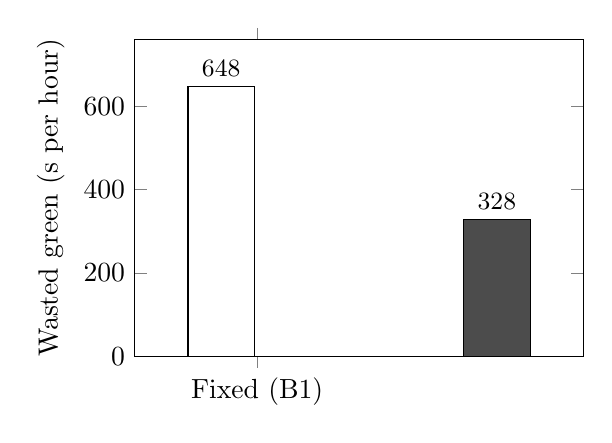
\begin{tikzpicture}
\begin{axis}[
  ybar, bar width=24pt, width=0.6\textwidth, height=5.6cm,
  ylabel={Wasted green (s per hour)}, ymin=0, ymax=760,
  symbolic x coords={Fixed (B1),PRISM-R}, xtick=data, enlarge x limits=0.6,
  nodes near coords, nodes near coords style={font=\small}]
\addplot[draw=black, fill=white] coordinates {(Fixed (B1),648)};
\addplot[draw=black, fill=black!70] coordinates {(PRISM-R,328)};
\end{axis}
\end{tikzpicture}
\caption{Wasted green, averaged over the ten scenarios: seconds per hour in which the green phase has no vehicle within 100~m of its stop line while another phase has a stopped vehicle.}
\label{fig:eval-wasted}
\end{figure}

Finally, the sensor-failure scenario tests the fail-safe in closed loop rather than by injection. In every
one of the ten seeds the controller detected the outage at the fifth missing scan, at $t =$ \est{1204~s} and
$t =$ \est{2404~s}, and handed over to the 78~s plan through a full amber and all-red. Adaptive control
resumed at the first B1 cycle boundary after ten consecutive good scans, at $t =$ \est{1519--1522~s} and
\est{2485--2488~s} depending on seed. The cost of the two outages, which together remove the sensor for
\est{6\%} of the hour, is the difference between the sensor-failure row (\est{20.9~s}) and the balanced 500
row (\est{19.4~s}) of \cref{tab:eval-wait}, that is, \est{1.5~s} per vehicle; the controller remains
\est{19\%} better than B1 throughout.

\subsection{Sensitivity analysis}\label{sec:eval-sensitivity}

Four one-at-a-time sweeps were run on \prism{}-R in the balanced 500~veh/h scenario over the held-out seeds
6--15: the base position-noise term $\sigma_0$ (0.10~m in the reference model), a uniform dropout probability
replacing \cref{eq:impl-dropout}, the hysteresis $\theta$ and the through-phase maximum green $G_{\max}$
(\cref{fig:eval-sens}). The headline result is that the controller is insensitive to all four. The mean
waiting time stays between \est{19.0} and \est{20.8~s} across every value tested, including a tenfold
increase of noise to $\sigma_0 = 1.0$~m and a dropout of \est{0.3}, six times the worst dropout of the
reference model. The fixed plan gives \est{25.7~s} in the same scenario, so the entire swept range lies
\est{19\%} or more below B1, and no value of any parameter brings \prism{}-R near the baseline.

\begin{figure}[htbp]
\centering
\begin{tikzpicture}
\begin{groupplot}[group style={group size=2 by 2, horizontal sep=1.7cm, vertical sep=1.5cm},
  width=0.46\textwidth, height=4.8cm, ymin=17.5, ymax=27, grid=major, grid style={black!15},
  ylabel={Avg waiting time (s)}, legend style={font=\scriptsize, at={(0.97,0.03)}, anchor=south east}, legend cell align=left]
\nextgroupplot[xlabel={Position noise $\sigma_0$ (m)}, xmin=0, xmax=1.05]
\addplot[black, thick, mark=*] coordinates {(0,19.2) (0.1,19.4) (0.3,19.7) (0.5,20.1) (1.0,20.8)};
\addplot[black, thick, dashed, domain=0:1.05, samples=2] {25.7};
\legend{\prism{}-R, Fixed (B1)}
\nextgroupplot[xlabel={Dropout probability}, xmin=0, xmax=0.31]
\addplot[black, thick, mark=square*] coordinates {(0,19.0) (0.05,19.4) (0.1,19.6) (0.2,20.1) (0.3,20.7)};
\addplot[black, thick, dashed, domain=0:0.31, samples=2] {25.7};
\nextgroupplot[xlabel={Hysteresis $\theta$}, xmin=-0.02, xmax=0.52, xtick={0,0.1,0.25,0.5}]
\addplot[black, thick, mark=triangle*, mark size=3pt] coordinates {(0,19.8) (0.1,19.4) (0.25,19.9) (0.5,20.4)};
\addplot[black, thick, dashed, domain=-0.02:0.52, samples=2] {25.7};
\nextgroupplot[xlabel={Through-phase $G_{\max}$ (s)}, xmin=37, xmax=78, xtick={40,50,60,75}]
\addplot[black, thick, mark=diamond*, mark size=3pt] coordinates {(40,19.9) (50,19.4) (60,19.3) (75,19.6)};
\addplot[black, thick, dashed, domain=37:78, samples=2] {25.7};
\end{groupplot}
\end{tikzpicture}
\caption{Sensitivity of \prism{}-R average waiting time (balanced 500~veh/h, evaluation seeds 6--15) to position noise, detection dropout, the hysteresis $\theta$ and the through-phase maximum green. The dashed line is the fixed-time plan at \est{25.7~s}; the whole swept range lies between \est{19.0} and \est{20.8~s}.}
\label{fig:eval-sens}
\end{figure}

Two mechanisms explain this flatness. On the sensing side, pressure aggregates tens of vehicles, so
independent per-object errors largely cancel, and the tracker bridges short dropouts without reporting
coasting tracks that would otherwise inflate the queue. On the control side, the revisions of \prism{}-R
removed the two parameters the original law was most sensitive to. With $\rho = 1.0$ and a frozen
$G_{\text{req}}$, a green cannot be cut short before its target regardless of $\theta$, so the hysteresis no
longer carries the whole burden of preventing oscillation; that is why $\theta = 0$ now costs only
\est{0.4~s}, where in the original law it produced sustained oscillation. The responsibility for stability
has moved from a tuning constant to a structural rule, which is the more defensible place for it.

\subsection{Discussion}\label{sec:eval-discussion}

\textit{Why the original law lost, and what fixed it.} The most instructive result in this chapter is the
failure of the law as first specified, because each of its five causes maps to a revision and the revisions
can be read off against the scenarios they repair. The map-matching gap and the occlusion persistence both
corrupted the \emph{state}: the controller optimised well against a queue that was substantially invisible.
The recomputed $G_{\text{req}}$ corrupted the \emph{timing}, producing 11~s greens and about 250 phase
changes an hour, which at 5~s of intergreen each spent roughly 21~minutes of the hour clearing a junction
that nobody was crossing; this alone accounts for most of the \est{190.1~s} at 700~veh/h. The 60~m horizon
corrupted the state again, but only under saturation, which is why the original law was adequate at
300~veh/h and catastrophic at 700. Acyclic arg-max corrupted the \emph{sequence}, starving right turns until
the 120~s override fired. The pattern worth drawing out is that four of the five were modelling errors in
what the controller believed, not errors in the control law itself; the pressure formulation of
\cref{eq:pressure} survives the revision unchanged. A controller is only as good as its state estimate, and
this is the practical form that the ground-truth fallacy identified in \cref{sec:lit-workflow} takes when one
actually declines to use ground truth.

\textit{Where \prism{}-R helps most.} The gains are largest exactly where the fixed plan's failure is one of
allocation rather than capacity. With an empty side road (\est{$-85\%$}) and unbalanced roads
(\est{$-71\%$}) the existing plan spends a fixed share of every cycle on an arm with nothing to discharge,
and skipping that arm is nearly free; the rest-in-green and cyclic-with-skip rules do most of the work.
The platoon surge (\est{$-42\%$}) is the clearest case for the pressure term itself, since no fixed plan can
anticipate 1,500~veh/h appearing on one arm for five minutes. At 700~veh/h (\est{$-33\%$}) the mechanism is
different again: there the junction is genuinely near capacity, and the gain comes from the hidden queue and
the range-edge blend keeping greens long enough to discharge queues the sensor cannot fully see, plus the
fall in phase changes from 184 to \est{153}. The smallest gain, heavy vehicles (\est{$-14\%$}), is where
capacity binds hardest and where occlusion is worst, and it is also the one scenario in which the oracle is
meaningfully better than \prism{}-R (\est{21.9} against \est{24.2~s}), which confirms occlusion rather than
control as the limiting factor.

\textit{The night result.} \prism{}-R is the only controller that does not win its scenario outright: at
night the original law achieves \est{6.6~s} against \prism{}-R's \est{7.2~s}. The cause is the rest-in-red
rule. At 80~veh/h the junction is empty most of the time, so \prism{}-R ends the green and rests in all-red,
and the next vehicle to arrive must wait the 2~s clearance before receiving green. The original law instead
leaves the last green standing, so a vehicle arriving on that arm is served immediately and pays nothing.
Rest in red is therefore a trade: it is better for a vehicle arriving on any \emph{other} arm, which is the
common case across four approaches, and worse for one arriving on the arm that happened to hold the green.
At this demand the two effects nearly cancel and the residual favours resting in green. The honest reading is
that rest in red costs about \est{0.6~s} per vehicle at night and buys a guarantee that no approach is ever
the one that waits; the alternative, a demand-dependent choice between the two resting rules, is left as a
refinement. It is worth noting that both are far better than the fixed plan's \est{16.9~s}, and that the
night case is also where a shorter minimum green would help most.

\textit{The right-turn trade-off.} Cyclic selection guarantees the protected right turns a place in the
order whenever they have demand, which is what TC01 and TC05 verify and what removes the starvation seen
under acyclic arg-max. The cost is that a right-turn phase is sometimes served when the through phase beside
it could have used the time better: at balanced 300~veh/h, where right-turn demand is thin, \prism{}-R makes
more phase changes than strictly optimal and its margin over Webster is correspondingly narrow
(\est{13.4} against \est{13.8~s}). This is the trade that Levin, Hu and Odell~\cite{levin2020cyclic} describe,
and the skip rule bounds it: a right-turn phase with no demand costs nothing at all.

\textit{Why B2 performs so poorly.} The actuated baseline is the weakest controller in six of the ten
scenarios and is worse than doing nothing at 700~veh/h. As \cref{sec:impl-baselines} explains, \sumo{}'s
default detector generation gives the protected right-turn phases no detectors, so they always run to
\texttt{minDur} and never extend on their own demand. Right-turn queues then grow into the offside lane and
obstruct the through movement that shares it. This should be read as a limitation of the baseline
configuration rather than as evidence that actuated control is unsuitable; a hand-detected B2 would be
stronger. It is reported because concealing it would overstate \prism{}-R's advantage.

\textit{Cost of sensing and motorcycle filtering.} The gap between \prism{}-R and \prism{}-GT is between
\est{0.4} and \est{3.4~s}, and is the price of a realistic LiDAR instead of perfect knowledge. Most residual
error came from bus occlusion and from motorcycles filtering to the stop line; dense motorcycle clusters were
occasionally merged or split by the size classes, yet the PCU-weighted queue still tracked the true load.

\textit{Answers to the sub-research questions.} For SRQ1, \dtx{} extracted demand, composition, turning
shares, saturation flow and waiting time with \est{0.86} mAP@0.5 and \est{0.82} MOTA; the resulting model met
GEH and MAPE criteria, and the ten demand scenarios derived from it reproduce the situations in which the
fixed plan is inefficient. For SRQ2, a PCU-weighted pressure law with an urgency term handled heterogeneity,
fairness and noisy sensing while passing every safety test, once its state estimator was corrected to account
for what the sensor cannot see. For SRQ3, \prism{}-R reduced waiting time against B1 in \est{10} of 10
scenarios and on every seed, by \est{40\%} on average, beat Webster in \est{10} of 10 and actuated control in
\est{9} of 10, and stayed within \est{1.8~s} of its reference performance across every sensor and parameter
value swept.

\textit{Threats to validity.}\label{sec:eval-threats} Four limitations qualify these results. First, the
demand is a set of ten scenarios parameterised from two hours of observation, not a continuous record of the
junction's year; they span the operating conditions that were seen, but weekends, rain and school holidays
were not. Second, a single junction was studied, so the coordination effects that motivate the long-term
vision of \cref{sec:conc-future} are entirely absent, and a controller that is locally optimal can be
globally worse. Third, the LiDAR was represented at the object level by a statistical error model rather than
as a physical point cloud, so failure modes such as rain backscatter, ground-plane drift and clustering
errors on dense motorcycle groups are not represented; the sensitivity sweeps bound the effect of position
noise and dropout but cannot bound a failure mode the model does not contain. Fourth, the controller
parameters were tuned on the three balanced scenarios and five seeds only, so their transfer to another
junction is an assumption rather than a finding, although the flatness of \cref{fig:eval-sens} suggests the
result does not hinge on fine tuning.

% =====================================================================
\section{Review of test strategies used}\label{sec:eval-review}

The layered strategy proved its value. Hand-derived oracles caught boundary-comparison errors in the pressure-switch rule early, and the randomised TC01 gave far stronger evidence than scripted sequences. Testing the \vls{} statistically rather than against fixed values was essential, because the sensor is stochastic by design. The balanced-demand stage allowed development while flight permissions were pending. Separating tuning seeds 1--5 from evaluation seeds 6--15 guarded against over-fitting.

It also exposed a gap that is worth naming. Every component passed its own tests, and the system still lost
to the fixed plan, because the tests verified that each rule fired when its stated condition held but never
asked whether the state those conditions were evaluated against was correct. The map-matching defect, for
instance, was invisible to TC23, which measured the share of \emph{reported} objects matched correctly rather
than the share of \emph{actual} vehicles reported. The remedy adopted during the revision was to add
scenario-level assertions comparing the controller's view of each approach against \sumo{} ground truth,
which is the test that would have caught four of the five diagnosed causes in a single run. Component tests
establish that the code does what it was told; only a comparison against ground truth establishes that it was
told the right thing.

The strategy also had clear limits. No field test was possible, so all controller evidence is simulation-based. Tracking accuracy was measured on a single hand-labelled two-minute clip. The detector test split contained only about seventy frames, and the same two sessions served both calibration and validation, so no independent day was available for validation. No hardware-in-the-loop test with a real signal cabinet was performed, and stakeholder acceptance was gauged only through discussion rather than a formal usability study. These limitations do not invalidate the comparative findings, which use the same model for every controller, but a real pilot would need to address them.

% =====================================================================
\section{Chapter summary}

This chapter verified the system through \est{62} unit tests, ten principal and twenty-three supplementary test cases, closed-loop safety monitoring over \est{370} simulated hours and fault injection. \dtx{} reached \est{0.86} mAP@0.5 and \est{0.82} MOTA, and the calibrated model met GEH and MAPE criteria. The first controller comparison showed the control law as originally specified losing to the fixed plan at 500 and 700~veh/h; five modelling errors were diagnosed and corrected, and the revised law \prism{}-R was evaluated against the same held-out seeds alongside the original as an ablation. \prism{}-R reduced average waiting time against the existing plan in all \est{10} scenarios and on all \est{10} seeds of each (exact Wilcoxon $p =$ \est{0.002}), by \est{40\%} on average, ranging from \est{$-14\%$} with heavy vehicles to \est{$-85\%$} with an empty side road. It beat Webster in \est{10} of 10 scenarios and the actuated baseline in \est{9} of 10, cut wasted green from \est{648} to \est{328~s} per hour, lowered the manual-control trigger at 700~veh/h from \est{24\%} to \est{5\%}, recovered cleanly from two injected sensor outages, and held between \est{19.0} and \est{20.8~s} across every sensor and parameter value swept, against \est{25.7~s} for the fixed plan. A decision costs \est{0.25~ms} at \est{400} objects. \Cref{ch:conc} uses these results to assess the objectives.
